\documentclass[10pt]{article}
\usepackage[margin=1cm]{geometry}
\geometry{a4paper}

\usepackage{fontawesome}
\usepackage[dvipsnames]{xcolor}

\usepackage{tikz}
\usetikzlibrary{patterns}
\usetikzlibrary{patterns.meta}

\pagestyle{empty}

\begin{document}

\begin{center}
\begin{tikzpicture}
  % PLAYER A
  \node[] at (-5,-0.5) {\parbox{5cm}{\centering \sffamily \Large \color{BrickRed} \textbf{Player A}}};
  \node[] at (-5,-1.25) {\parbox{5cm}{\centering \sffamily \large \color{BrickRed} \textbf{
  (Pick one to solve)	
  }}};
  % PLAYER A, NUMBER 1
  \node[] at (-5,-2.75) {\parbox{5cm}{\sffamily \large \color{BrickRed}
  \textbf{Level 1} \hfill {\faGear}%
  }};
  \node[] at (-5,-6) {%
  \begin{tikzpicture}[scale=0.6]
\node[anchor=center] at (0.5,8.5) {};
\node[anchor=center] at (0.5,7.5) {\Large 9};
\node[anchor=center] at (0.5,6.5) {};
\node[anchor=center] at (0.5,5.5) {};
\node[anchor=center] at (0.5,4.5) {\Large 7};
\node[anchor=center] at (0.5,3.5) {};
\node[anchor=center] at (0.5,2.5) {\Large 5};
\node[anchor=center] at (0.5,1.5) {\Large 2};
\node[anchor=center] at (0.5,0.5) {};
\node[anchor=center] at (1.5,8.5) {};
\node[anchor=center] at (1.5,7.5) {\Large 5};
\node[anchor=center] at (1.5,6.5) {};
\node[anchor=center] at (1.5,5.5) {\Large 1};
\node[anchor=center] at (1.5,4.5) {};
\node[anchor=center] at (1.5,3.5) {};
\node[anchor=center] at (1.5,2.5) {};
\node[anchor=center] at (1.5,1.5) {};
\node[anchor=center] at (1.5,0.5) {};
\node[anchor=center] at (2.5,8.5) {\Large 8};
\node[anchor=center] at (2.5,7.5) {};
\node[anchor=center] at (2.5,6.5) {\Large 2};
\node[anchor=center] at (2.5,5.5) {};
\node[anchor=center] at (2.5,4.5) {};
\node[anchor=center] at (2.5,3.5) {};
\node[anchor=center] at (2.5,2.5) {};
\node[anchor=center] at (2.5,1.5) {\Large 7};
\node[anchor=center] at (2.5,0.5) {};
\node[anchor=center] at (3.5,8.5) {};
\node[anchor=center] at (3.5,7.5) {};
\node[anchor=center] at (3.5,6.5) {\Large 7};
\node[anchor=center] at (3.5,5.5) {\Large 6};
\node[anchor=center] at (3.5,4.5) {\Large 1};
\node[anchor=center] at (3.5,3.5) {};
\node[anchor=center] at (3.5,2.5) {};
\node[anchor=center] at (3.5,1.5) {};
\node[anchor=center] at (3.5,0.5) {};
\node[anchor=center] at (4.5,8.5) {\Large 5};
\node[anchor=center] at (4.5,7.5) {};
\node[anchor=center] at (4.5,6.5) {};
\node[anchor=center] at (4.5,5.5) {\Large 9};
\node[anchor=center] at (4.5,4.5) {};
\node[anchor=center] at (4.5,3.5) {};
\node[anchor=center] at (4.5,2.5) {\Large 2};
\node[anchor=center, minimum width=17pt, minimum height=17pt, pattern=north west lines, pattern color=BrickRed!40] at (4.5,1.5) {};
\node[anchor=center] at (4.5,0.5) {};
\node[anchor=center] at (5.5,8.5) {};
\node[anchor=center] at (5.5,7.5) {};
\node[anchor=center] at (5.5,6.5) {};
\node[anchor=center] at (5.5,5.5) {};
\node[anchor=center] at (5.5,4.5) {};
\node[anchor=center] at (5.5,3.5) {\Large 4};
\node[anchor=center] at (5.5,2.5) {\Large 8};
\node[anchor=center] at (5.5,1.5) {};
\node[anchor=center] at (5.5,0.5) {};
\node[anchor=center] at (6.5,8.5) {};
\node[anchor=center] at (6.5,7.5) {\Large 4};
\node[anchor=center] at (6.5,6.5) {};
\node[anchor=center] at (6.5,5.5) {};
\node[anchor=center] at (6.5,4.5) {};
\node[anchor=center] at (6.5,3.5) {\Large 9};
\node[anchor=center] at (6.5,2.5) {};
\node[anchor=center] at (6.5,1.5) {};
\node[anchor=center] at (6.5,0.5) {};
\node[anchor=center] at (7.5,8.5) {};
\node[anchor=center, minimum width=17pt, minimum height=17pt, pattern={Lines[distance=1.5pt,yshift=0.85pt]}, pattern color=NavyBlue!60] at (7.5,7.5) {};
\node[anchor=center] at (7.5,6.5) {\Large 9};
\node[anchor=center] at (7.5,5.5) {\Large 5};
\node[anchor=center] at (7.5,4.5) {\Large 6};
\node[anchor=center] at (7.5,3.5) {};
\node[anchor=center] at (7.5,2.5) {};
\node[anchor=center] at (7.5,1.5) {};
\node[anchor=center] at (7.5,0.5) {};
\node[anchor=center] at (8.5,8.5) {};
\node[anchor=center] at (8.5,7.5) {};
\node[anchor=center] at (8.5,6.5) {};
\node[anchor=center] at (8.5,5.5) {\Large 7};
\node[anchor=center] at (8.5,4.5) {};
\node[anchor=center] at (8.5,3.5) {};
\node[anchor=center] at (8.5,2.5) {\Large 6};
\node[anchor=center] at (8.5,1.5) {\Large 8};
\node[anchor=center] at (8.5,0.5) {};

        \draw[ultra thick, scale=3] (0, 0) grid (3, 3);
        \draw (0, 0) grid (9, 9);
        \end{tikzpicture}%
    
        % short form: 008050000950000400002700090010690057700100060000004900500028006207000008000000000
    %
  };
  % PLAYER A, NUMBER 2
  \node[] at (-5,-10.75) {\parbox{5cm}{\sffamily \large \color{BrickRed}
  \textbf{Level 2} \hfill {\faGear\ \faGear}%
  }};
  \node[] at (-5,-14) {%
  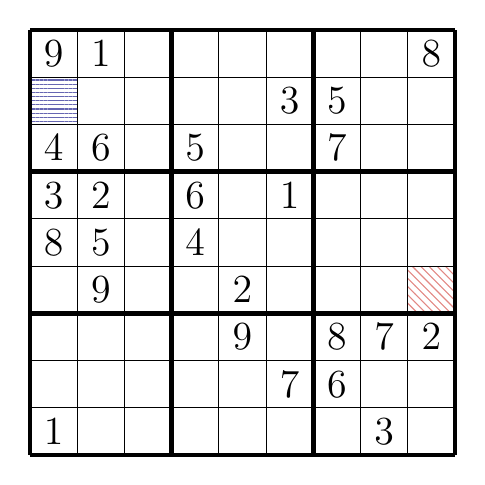
\begin{tikzpicture}[scale=0.6]
\node[anchor=center] at (0.5,8.5) {\Large 9};
\node[anchor=center, minimum width=17pt, minimum height=17pt, pattern={Lines[distance=1.5pt,yshift=0.85pt]}, pattern color=NavyBlue!60] at (0.5,7.5) {};
\node[anchor=center] at (0.5,6.5) {\Large 4};
\node[anchor=center] at (0.5,5.5) {\Large 3};
\node[anchor=center] at (0.5,4.5) {\Large 8};
\node[anchor=center] at (0.5,3.5) {};
\node[anchor=center] at (0.5,2.5) {};
\node[anchor=center] at (0.5,1.5) {};
\node[anchor=center] at (0.5,0.5) {\Large 1};
\node[anchor=center] at (1.5,8.5) {\Large 1};
\node[anchor=center] at (1.5,7.5) {};
\node[anchor=center] at (1.5,6.5) {\Large 6};
\node[anchor=center] at (1.5,5.5) {\Large 2};
\node[anchor=center] at (1.5,4.5) {\Large 5};
\node[anchor=center] at (1.5,3.5) {\Large 9};
\node[anchor=center] at (1.5,2.5) {};
\node[anchor=center] at (1.5,1.5) {};
\node[anchor=center] at (1.5,0.5) {};
\node[anchor=center] at (2.5,8.5) {};
\node[anchor=center] at (2.5,7.5) {};
\node[anchor=center] at (2.5,6.5) {};
\node[anchor=center] at (2.5,5.5) {};
\node[anchor=center] at (2.5,4.5) {};
\node[anchor=center] at (2.5,3.5) {};
\node[anchor=center] at (2.5,2.5) {};
\node[anchor=center] at (2.5,1.5) {};
\node[anchor=center] at (2.5,0.5) {};
\node[anchor=center] at (3.5,8.5) {};
\node[anchor=center] at (3.5,7.5) {};
\node[anchor=center] at (3.5,6.5) {\Large 5};
\node[anchor=center] at (3.5,5.5) {\Large 6};
\node[anchor=center] at (3.5,4.5) {\Large 4};
\node[anchor=center] at (3.5,3.5) {};
\node[anchor=center] at (3.5,2.5) {};
\node[anchor=center] at (3.5,1.5) {};
\node[anchor=center] at (3.5,0.5) {};
\node[anchor=center] at (4.5,8.5) {};
\node[anchor=center] at (4.5,7.5) {};
\node[anchor=center] at (4.5,6.5) {};
\node[anchor=center] at (4.5,5.5) {};
\node[anchor=center] at (4.5,4.5) {};
\node[anchor=center] at (4.5,3.5) {\Large 2};
\node[anchor=center] at (4.5,2.5) {\Large 9};
\node[anchor=center] at (4.5,1.5) {};
\node[anchor=center] at (4.5,0.5) {};
\node[anchor=center] at (5.5,8.5) {};
\node[anchor=center] at (5.5,7.5) {\Large 3};
\node[anchor=center] at (5.5,6.5) {};
\node[anchor=center] at (5.5,5.5) {\Large 1};
\node[anchor=center] at (5.5,4.5) {};
\node[anchor=center] at (5.5,3.5) {};
\node[anchor=center] at (5.5,2.5) {};
\node[anchor=center] at (5.5,1.5) {\Large 7};
\node[anchor=center] at (5.5,0.5) {};
\node[anchor=center] at (6.5,8.5) {};
\node[anchor=center] at (6.5,7.5) {\Large 5};
\node[anchor=center] at (6.5,6.5) {\Large 7};
\node[anchor=center] at (6.5,5.5) {};
\node[anchor=center] at (6.5,4.5) {};
\node[anchor=center] at (6.5,3.5) {};
\node[anchor=center] at (6.5,2.5) {\Large 8};
\node[anchor=center] at (6.5,1.5) {\Large 6};
\node[anchor=center] at (6.5,0.5) {};
\node[anchor=center] at (7.5,8.5) {};
\node[anchor=center] at (7.5,7.5) {};
\node[anchor=center] at (7.5,6.5) {};
\node[anchor=center] at (7.5,5.5) {};
\node[anchor=center] at (7.5,4.5) {};
\node[anchor=center] at (7.5,3.5) {};
\node[anchor=center] at (7.5,2.5) {\Large 7};
\node[anchor=center] at (7.5,1.5) {};
\node[anchor=center] at (7.5,0.5) {\Large 3};
\node[anchor=center] at (8.5,8.5) {\Large 8};
\node[anchor=center] at (8.5,7.5) {};
\node[anchor=center] at (8.5,6.5) {};
\node[anchor=center] at (8.5,5.5) {};
\node[anchor=center] at (8.5,4.5) {};
\node[anchor=center, minimum width=17pt, minimum height=17pt, pattern=north west lines, pattern color=BrickRed!40] at (8.5,3.5) {};
\node[anchor=center] at (8.5,2.5) {\Large 2};
\node[anchor=center] at (8.5,1.5) {};
\node[anchor=center] at (8.5,0.5) {};

        \draw[ultra thick, scale=3] (0, 0) grid (3, 3);
        \draw (0, 0) grid (9, 9);
        \end{tikzpicture}%
    
        % short form: 910000008000003500460500700320601000850400000090020000000090872000007600100000030
    %
  };
  % PLAYER A, NUMBER 3
  \node[] at (-5,-18.75) {\parbox{5cm}{\sffamily \large \color{BrickRed}
  \textbf{Level 3} \hfill {\faGear\ \faGear\ \faGear}%
  }};
  \node[] at (-5,-22) {%
  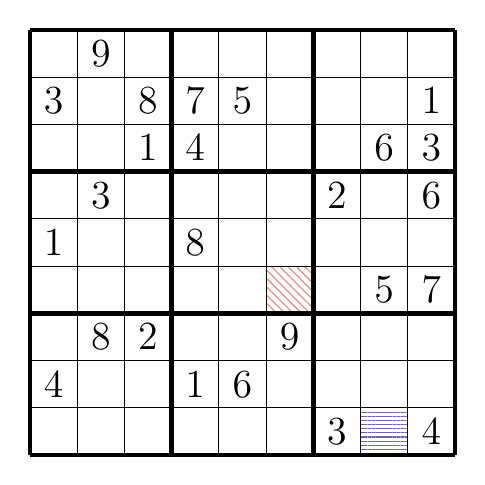
\begin{tikzpicture}[scale=0.6]
\node[anchor=center] at (0.5,8.5) {};
\node[anchor=center] at (0.5,7.5) {\Large 3};
\node[anchor=center] at (0.5,6.5) {};
\node[anchor=center] at (0.5,5.5) {};
\node[anchor=center] at (0.5,4.5) {\Large 1};
\node[anchor=center] at (0.5,3.5) {};
\node[anchor=center] at (0.5,2.5) {};
\node[anchor=center] at (0.5,1.5) {\Large 4};
\node[anchor=center] at (0.5,0.5) {};
\node[anchor=center] at (1.5,8.5) {\Large 9};
\node[anchor=center] at (1.5,7.5) {};
\node[anchor=center] at (1.5,6.5) {};
\node[anchor=center] at (1.5,5.5) {\Large 3};
\node[anchor=center] at (1.5,4.5) {};
\node[anchor=center] at (1.5,3.5) {};
\node[anchor=center] at (1.5,2.5) {\Large 8};
\node[anchor=center] at (1.5,1.5) {};
\node[anchor=center] at (1.5,0.5) {};
\node[anchor=center] at (2.5,8.5) {};
\node[anchor=center] at (2.5,7.5) {\Large 8};
\node[anchor=center] at (2.5,6.5) {\Large 1};
\node[anchor=center] at (2.5,5.5) {};
\node[anchor=center] at (2.5,4.5) {};
\node[anchor=center] at (2.5,3.5) {};
\node[anchor=center] at (2.5,2.5) {\Large 2};
\node[anchor=center] at (2.5,1.5) {};
\node[anchor=center] at (2.5,0.5) {};
\node[anchor=center] at (3.5,8.5) {};
\node[anchor=center] at (3.5,7.5) {\Large 7};
\node[anchor=center] at (3.5,6.5) {\Large 4};
\node[anchor=center] at (3.5,5.5) {};
\node[anchor=center] at (3.5,4.5) {\Large 8};
\node[anchor=center] at (3.5,3.5) {};
\node[anchor=center] at (3.5,2.5) {};
\node[anchor=center] at (3.5,1.5) {\Large 1};
\node[anchor=center] at (3.5,0.5) {};
\node[anchor=center] at (4.5,8.5) {};
\node[anchor=center] at (4.5,7.5) {\Large 5};
\node[anchor=center] at (4.5,6.5) {};
\node[anchor=center] at (4.5,5.5) {};
\node[anchor=center] at (4.5,4.5) {};
\node[anchor=center] at (4.5,3.5) {};
\node[anchor=center] at (4.5,2.5) {};
\node[anchor=center] at (4.5,1.5) {\Large 6};
\node[anchor=center] at (4.5,0.5) {};
\node[anchor=center] at (5.5,8.5) {};
\node[anchor=center] at (5.5,7.5) {};
\node[anchor=center] at (5.5,6.5) {};
\node[anchor=center] at (5.5,5.5) {};
\node[anchor=center] at (5.5,4.5) {};
\node[anchor=center, minimum width=17pt, minimum height=17pt, pattern=north west lines, pattern color=BrickRed!40] at (5.5,3.5) {};
\node[anchor=center] at (5.5,2.5) {\Large 9};
\node[anchor=center] at (5.5,1.5) {};
\node[anchor=center] at (5.5,0.5) {};
\node[anchor=center] at (6.5,8.5) {};
\node[anchor=center] at (6.5,7.5) {};
\node[anchor=center] at (6.5,6.5) {};
\node[anchor=center] at (6.5,5.5) {\Large 2};
\node[anchor=center] at (6.5,4.5) {};
\node[anchor=center] at (6.5,3.5) {};
\node[anchor=center] at (6.5,2.5) {};
\node[anchor=center] at (6.5,1.5) {};
\node[anchor=center] at (6.5,0.5) {\Large 3};
\node[anchor=center] at (7.5,8.5) {};
\node[anchor=center] at (7.5,7.5) {};
\node[anchor=center] at (7.5,6.5) {\Large 6};
\node[anchor=center] at (7.5,5.5) {};
\node[anchor=center] at (7.5,4.5) {};
\node[anchor=center] at (7.5,3.5) {\Large 5};
\node[anchor=center] at (7.5,2.5) {};
\node[anchor=center] at (7.5,1.5) {};
\node[anchor=center, minimum width=17pt, minimum height=17pt, pattern={Lines[distance=1.5pt,yshift=0.85pt]}, pattern color=NavyBlue!60] at (7.5,0.5) {};
\node[anchor=center] at (8.5,8.5) {};
\node[anchor=center] at (8.5,7.5) {\Large 1};
\node[anchor=center] at (8.5,6.5) {\Large 3};
\node[anchor=center] at (8.5,5.5) {\Large 6};
\node[anchor=center] at (8.5,4.5) {};
\node[anchor=center] at (8.5,3.5) {\Large 7};
\node[anchor=center] at (8.5,2.5) {};
\node[anchor=center] at (8.5,1.5) {};
\node[anchor=center] at (8.5,0.5) {\Large 4};

        \draw[ultra thick, scale=3] (0, 0) grid (3, 3);
        \draw (0, 0) grid (9, 9);
        \end{tikzpicture}%
    
        % short form: 090000000308750001001400063030000206100800000000000057082009000400160000000000304
    %
  };
  %
  \node[] at (-5,-26.5) {\parbox{5cm}{\centering \sffamily Puzzle~\#%
  1-10-A%
  }};
  % PLAYER B
  \node[] at (5,-0.5) {\parbox{5cm}{\centering \sffamily \Large \color{BrickRed} \textbf{Player B}}};
  \node[] at (5,-1.25) {\parbox{5cm}{\centering \sffamily \large \color{BrickRed} \textbf{
  (Pick one to solve)
  }}};
  % PLAYER B, NUMBER 1
  \node[] at (5,-2.75) {\parbox{5cm}{\sffamily \large \color{BrickRed}
  \textbf{Level 2} \hfill {\faGear\ \faGear}%
  }};
  \node[] at (5,-6) {%
  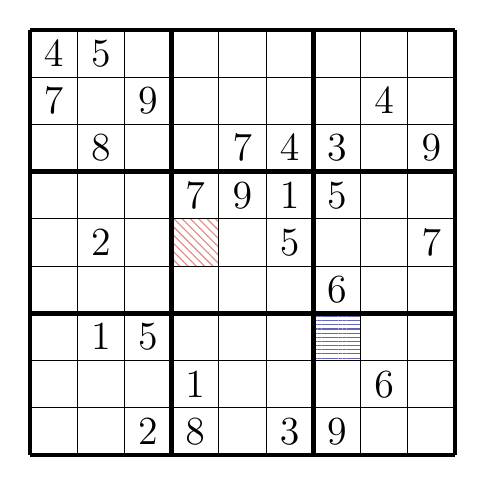
\begin{tikzpicture}[scale=0.6]
\node[anchor=center] at (0.5,8.5) {\Large 4};
\node[anchor=center] at (0.5,7.5) {\Large 7};
\node[anchor=center] at (0.5,6.5) {};
\node[anchor=center] at (0.5,5.5) {};
\node[anchor=center] at (0.5,4.5) {};
\node[anchor=center] at (0.5,3.5) {};
\node[anchor=center] at (0.5,2.5) {};
\node[anchor=center] at (0.5,1.5) {};
\node[anchor=center] at (0.5,0.5) {};
\node[anchor=center] at (1.5,8.5) {\Large 5};
\node[anchor=center] at (1.5,7.5) {};
\node[anchor=center] at (1.5,6.5) {\Large 8};
\node[anchor=center] at (1.5,5.5) {};
\node[anchor=center] at (1.5,4.5) {\Large 2};
\node[anchor=center] at (1.5,3.5) {};
\node[anchor=center] at (1.5,2.5) {\Large 1};
\node[anchor=center] at (1.5,1.5) {};
\node[anchor=center] at (1.5,0.5) {};
\node[anchor=center] at (2.5,8.5) {};
\node[anchor=center] at (2.5,7.5) {\Large 9};
\node[anchor=center] at (2.5,6.5) {};
\node[anchor=center] at (2.5,5.5) {};
\node[anchor=center] at (2.5,4.5) {};
\node[anchor=center] at (2.5,3.5) {};
\node[anchor=center] at (2.5,2.5) {\Large 5};
\node[anchor=center] at (2.5,1.5) {};
\node[anchor=center] at (2.5,0.5) {\Large 2};
\node[anchor=center] at (3.5,8.5) {};
\node[anchor=center] at (3.5,7.5) {};
\node[anchor=center] at (3.5,6.5) {};
\node[anchor=center] at (3.5,5.5) {\Large 7};
\node[anchor=center, minimum width=17pt, minimum height=17pt, pattern=north west lines, pattern color=BrickRed!40] at (3.5,4.5) {};
\node[anchor=center] at (3.5,3.5) {};
\node[anchor=center] at (3.5,2.5) {};
\node[anchor=center] at (3.5,1.5) {\Large 1};
\node[anchor=center] at (3.5,0.5) {\Large 8};
\node[anchor=center] at (4.5,8.5) {};
\node[anchor=center] at (4.5,7.5) {};
\node[anchor=center] at (4.5,6.5) {\Large 7};
\node[anchor=center] at (4.5,5.5) {\Large 9};
\node[anchor=center] at (4.5,4.5) {};
\node[anchor=center] at (4.5,3.5) {};
\node[anchor=center] at (4.5,2.5) {};
\node[anchor=center] at (4.5,1.5) {};
\node[anchor=center] at (4.5,0.5) {};
\node[anchor=center] at (5.5,8.5) {};
\node[anchor=center] at (5.5,7.5) {};
\node[anchor=center] at (5.5,6.5) {\Large 4};
\node[anchor=center] at (5.5,5.5) {\Large 1};
\node[anchor=center] at (5.5,4.5) {\Large 5};
\node[anchor=center] at (5.5,3.5) {};
\node[anchor=center] at (5.5,2.5) {};
\node[anchor=center] at (5.5,1.5) {};
\node[anchor=center] at (5.5,0.5) {\Large 3};
\node[anchor=center] at (6.5,8.5) {};
\node[anchor=center] at (6.5,7.5) {};
\node[anchor=center] at (6.5,6.5) {\Large 3};
\node[anchor=center] at (6.5,5.5) {\Large 5};
\node[anchor=center] at (6.5,4.5) {};
\node[anchor=center] at (6.5,3.5) {\Large 6};
\node[anchor=center, minimum width=17pt, minimum height=17pt, pattern={Lines[distance=1.5pt,yshift=0.85pt]}, pattern color=NavyBlue!60] at (6.5,2.5) {};
\node[anchor=center] at (6.5,1.5) {};
\node[anchor=center] at (6.5,0.5) {\Large 9};
\node[anchor=center] at (7.5,8.5) {};
\node[anchor=center] at (7.5,7.5) {\Large 4};
\node[anchor=center] at (7.5,6.5) {};
\node[anchor=center] at (7.5,5.5) {};
\node[anchor=center] at (7.5,4.5) {};
\node[anchor=center] at (7.5,3.5) {};
\node[anchor=center] at (7.5,2.5) {};
\node[anchor=center] at (7.5,1.5) {\Large 6};
\node[anchor=center] at (7.5,0.5) {};
\node[anchor=center] at (8.5,8.5) {};
\node[anchor=center] at (8.5,7.5) {};
\node[anchor=center] at (8.5,6.5) {\Large 9};
\node[anchor=center] at (8.5,5.5) {};
\node[anchor=center] at (8.5,4.5) {\Large 7};
\node[anchor=center] at (8.5,3.5) {};
\node[anchor=center] at (8.5,2.5) {};
\node[anchor=center] at (8.5,1.5) {};
\node[anchor=center] at (8.5,0.5) {};

        \draw[ultra thick, scale=3] (0, 0) grid (3, 3);
        \draw (0, 0) grid (9, 9);
        \end{tikzpicture}%
    
        % short form: 450000000709000040080074309000791500020005007000000600015000000000100060002803900
    %
  };
  % PLAYER B, NUMBER 2
  \node[] at (5,-10.75) {\parbox{5cm}{\sffamily \large \color{BrickRed}
  \textbf{Level 3} \hfill {\faGear\ \faGear\ \faGear}%
  }};
  \node[] at (5,-14) {%
  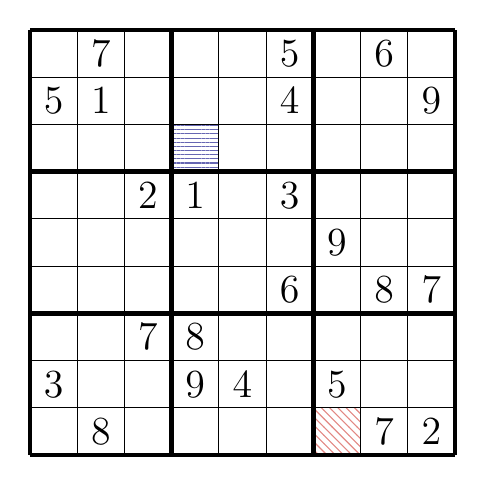
\begin{tikzpicture}[scale=0.6]
\node[anchor=center] at (0.5,8.5) {};
\node[anchor=center] at (0.5,7.5) {\Large 5};
\node[anchor=center] at (0.5,6.5) {};
\node[anchor=center] at (0.5,5.5) {};
\node[anchor=center] at (0.5,4.5) {};
\node[anchor=center] at (0.5,3.5) {};
\node[anchor=center] at (0.5,2.5) {};
\node[anchor=center] at (0.5,1.5) {\Large 3};
\node[anchor=center] at (0.5,0.5) {};
\node[anchor=center] at (1.5,8.5) {\Large 7};
\node[anchor=center] at (1.5,7.5) {\Large 1};
\node[anchor=center] at (1.5,6.5) {};
\node[anchor=center] at (1.5,5.5) {};
\node[anchor=center] at (1.5,4.5) {};
\node[anchor=center] at (1.5,3.5) {};
\node[anchor=center] at (1.5,2.5) {};
\node[anchor=center] at (1.5,1.5) {};
\node[anchor=center] at (1.5,0.5) {\Large 8};
\node[anchor=center] at (2.5,8.5) {};
\node[anchor=center] at (2.5,7.5) {};
\node[anchor=center] at (2.5,6.5) {};
\node[anchor=center] at (2.5,5.5) {\Large 2};
\node[anchor=center] at (2.5,4.5) {};
\node[anchor=center] at (2.5,3.5) {};
\node[anchor=center] at (2.5,2.5) {\Large 7};
\node[anchor=center] at (2.5,1.5) {};
\node[anchor=center] at (2.5,0.5) {};
\node[anchor=center] at (3.5,8.5) {};
\node[anchor=center] at (3.5,7.5) {};
\node[anchor=center, minimum width=17pt, minimum height=17pt, pattern={Lines[distance=1.5pt,yshift=0.85pt]}, pattern color=NavyBlue!60] at (3.5,6.5) {};
\node[anchor=center] at (3.5,5.5) {\Large 1};
\node[anchor=center] at (3.5,4.5) {};
\node[anchor=center] at (3.5,3.5) {};
\node[anchor=center] at (3.5,2.5) {\Large 8};
\node[anchor=center] at (3.5,1.5) {\Large 9};
\node[anchor=center] at (3.5,0.5) {};
\node[anchor=center] at (4.5,8.5) {};
\node[anchor=center] at (4.5,7.5) {};
\node[anchor=center] at (4.5,6.5) {};
\node[anchor=center] at (4.5,5.5) {};
\node[anchor=center] at (4.5,4.5) {};
\node[anchor=center] at (4.5,3.5) {};
\node[anchor=center] at (4.5,2.5) {};
\node[anchor=center] at (4.5,1.5) {\Large 4};
\node[anchor=center] at (4.5,0.5) {};
\node[anchor=center] at (5.5,8.5) {\Large 5};
\node[anchor=center] at (5.5,7.5) {\Large 4};
\node[anchor=center] at (5.5,6.5) {};
\node[anchor=center] at (5.5,5.5) {\Large 3};
\node[anchor=center] at (5.5,4.5) {};
\node[anchor=center] at (5.5,3.5) {\Large 6};
\node[anchor=center] at (5.5,2.5) {};
\node[anchor=center] at (5.5,1.5) {};
\node[anchor=center] at (5.5,0.5) {};
\node[anchor=center] at (6.5,8.5) {};
\node[anchor=center] at (6.5,7.5) {};
\node[anchor=center] at (6.5,6.5) {};
\node[anchor=center] at (6.5,5.5) {};
\node[anchor=center] at (6.5,4.5) {\Large 9};
\node[anchor=center] at (6.5,3.5) {};
\node[anchor=center] at (6.5,2.5) {};
\node[anchor=center] at (6.5,1.5) {\Large 5};
\node[anchor=center, minimum width=17pt, minimum height=17pt, pattern=north west lines, pattern color=BrickRed!40] at (6.5,0.5) {};
\node[anchor=center] at (7.5,8.5) {\Large 6};
\node[anchor=center] at (7.5,7.5) {};
\node[anchor=center] at (7.5,6.5) {};
\node[anchor=center] at (7.5,5.5) {};
\node[anchor=center] at (7.5,4.5) {};
\node[anchor=center] at (7.5,3.5) {\Large 8};
\node[anchor=center] at (7.5,2.5) {};
\node[anchor=center] at (7.5,1.5) {};
\node[anchor=center] at (7.5,0.5) {\Large 7};
\node[anchor=center] at (8.5,8.5) {};
\node[anchor=center] at (8.5,7.5) {\Large 9};
\node[anchor=center] at (8.5,6.5) {};
\node[anchor=center] at (8.5,5.5) {};
\node[anchor=center] at (8.5,4.5) {};
\node[anchor=center] at (8.5,3.5) {\Large 7};
\node[anchor=center] at (8.5,2.5) {};
\node[anchor=center] at (8.5,1.5) {};
\node[anchor=center] at (8.5,0.5) {\Large 2};

        \draw[ultra thick, scale=3] (0, 0) grid (3, 3);
        \draw (0, 0) grid (9, 9);
        \end{tikzpicture}%
    
        % short form: 070005060510004009000000000002103000000000900000006087007800000300940500080000072
    %
  };
  % PLAYER B, NUMBER 3
  \node[] at (5,-18.75) %{\parbox{5cm}{\sffamily \large \color{BrickRed} }};
  {\parbox{5cm}{\sffamily \large \color{BrickRed}
  \textbf{Level 4} \hfill {\faGear\ \faGear\ \faGear\ \faGear}%
  }};
  \node[] at (5,-22) {%
  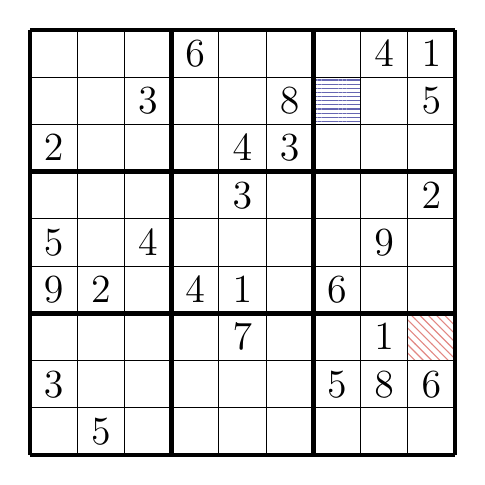
\begin{tikzpicture}[scale=0.6]
\node[anchor=center] at (0.5,8.5) {};
\node[anchor=center] at (0.5,7.5) {};
\node[anchor=center] at (0.5,6.5) {\Large 2};
\node[anchor=center] at (0.5,5.5) {};
\node[anchor=center] at (0.5,4.5) {\Large 5};
\node[anchor=center] at (0.5,3.5) {\Large 9};
\node[anchor=center] at (0.5,2.5) {};
\node[anchor=center] at (0.5,1.5) {\Large 3};
\node[anchor=center] at (0.5,0.5) {};
\node[anchor=center] at (1.5,8.5) {};
\node[anchor=center] at (1.5,7.5) {};
\node[anchor=center] at (1.5,6.5) {};
\node[anchor=center] at (1.5,5.5) {};
\node[anchor=center] at (1.5,4.5) {};
\node[anchor=center] at (1.5,3.5) {\Large 2};
\node[anchor=center] at (1.5,2.5) {};
\node[anchor=center] at (1.5,1.5) {};
\node[anchor=center] at (1.5,0.5) {\Large 5};
\node[anchor=center] at (2.5,8.5) {};
\node[anchor=center] at (2.5,7.5) {\Large 3};
\node[anchor=center] at (2.5,6.5) {};
\node[anchor=center] at (2.5,5.5) {};
\node[anchor=center] at (2.5,4.5) {\Large 4};
\node[anchor=center] at (2.5,3.5) {};
\node[anchor=center] at (2.5,2.5) {};
\node[anchor=center] at (2.5,1.5) {};
\node[anchor=center] at (2.5,0.5) {};
\node[anchor=center] at (3.5,8.5) {\Large 6};
\node[anchor=center] at (3.5,7.5) {};
\node[anchor=center] at (3.5,6.5) {};
\node[anchor=center] at (3.5,5.5) {};
\node[anchor=center] at (3.5,4.5) {};
\node[anchor=center] at (3.5,3.5) {\Large 4};
\node[anchor=center] at (3.5,2.5) {};
\node[anchor=center] at (3.5,1.5) {};
\node[anchor=center] at (3.5,0.5) {};
\node[anchor=center] at (4.5,8.5) {};
\node[anchor=center] at (4.5,7.5) {};
\node[anchor=center] at (4.5,6.5) {\Large 4};
\node[anchor=center] at (4.5,5.5) {\Large 3};
\node[anchor=center] at (4.5,4.5) {};
\node[anchor=center] at (4.5,3.5) {\Large 1};
\node[anchor=center] at (4.5,2.5) {\Large 7};
\node[anchor=center] at (4.5,1.5) {};
\node[anchor=center] at (4.5,0.5) {};
\node[anchor=center] at (5.5,8.5) {};
\node[anchor=center] at (5.5,7.5) {\Large 8};
\node[anchor=center] at (5.5,6.5) {\Large 3};
\node[anchor=center] at (5.5,5.5) {};
\node[anchor=center] at (5.5,4.5) {};
\node[anchor=center] at (5.5,3.5) {};
\node[anchor=center] at (5.5,2.5) {};
\node[anchor=center] at (5.5,1.5) {};
\node[anchor=center] at (5.5,0.5) {};
\node[anchor=center] at (6.5,8.5) {};
\node[anchor=center, minimum width=17pt, minimum height=17pt, pattern={Lines[distance=1.5pt,yshift=0.85pt]}, pattern color=NavyBlue!60] at (6.5,7.5) {};
\node[anchor=center] at (6.5,6.5) {};
\node[anchor=center] at (6.5,5.5) {};
\node[anchor=center] at (6.5,4.5) {};
\node[anchor=center] at (6.5,3.5) {\Large 6};
\node[anchor=center] at (6.5,2.5) {};
\node[anchor=center] at (6.5,1.5) {\Large 5};
\node[anchor=center] at (6.5,0.5) {};
\node[anchor=center] at (7.5,8.5) {\Large 4};
\node[anchor=center] at (7.5,7.5) {};
\node[anchor=center] at (7.5,6.5) {};
\node[anchor=center] at (7.5,5.5) {};
\node[anchor=center] at (7.5,4.5) {\Large 9};
\node[anchor=center] at (7.5,3.5) {};
\node[anchor=center] at (7.5,2.5) {\Large 1};
\node[anchor=center] at (7.5,1.5) {\Large 8};
\node[anchor=center] at (7.5,0.5) {};
\node[anchor=center] at (8.5,8.5) {\Large 1};
\node[anchor=center] at (8.5,7.5) {\Large 5};
\node[anchor=center] at (8.5,6.5) {};
\node[anchor=center] at (8.5,5.5) {\Large 2};
\node[anchor=center] at (8.5,4.5) {};
\node[anchor=center] at (8.5,3.5) {};
\node[anchor=center, minimum width=17pt, minimum height=17pt, pattern=north west lines, pattern color=BrickRed!40] at (8.5,2.5) {};
\node[anchor=center] at (8.5,1.5) {\Large 6};
\node[anchor=center] at (8.5,0.5) {};

        \draw[ultra thick, scale=3] (0, 0) grid (3, 3);
        \draw (0, 0) grid (9, 9);
        \end{tikzpicture}%
    
        % short form: 000600041003008005200043000000030002504000090920410600000070010300000586050000000
    %
  };
  %
  \node[] at (5,-26.5) {\parbox{5cm}{\centering \sffamily Puzzle~\#%
  1-10-B%
  }};
  %
  \draw[] (0,0.5) edge[ultra thick, dashed] (0,-27);
  \node[fill=white,inner sep=0pt] at (0,-26.2) {\rotatebox{90}{\Huge \faScissors}};
  %
\end{tikzpicture}
\end{center}

\pagebreak
\begin{center}
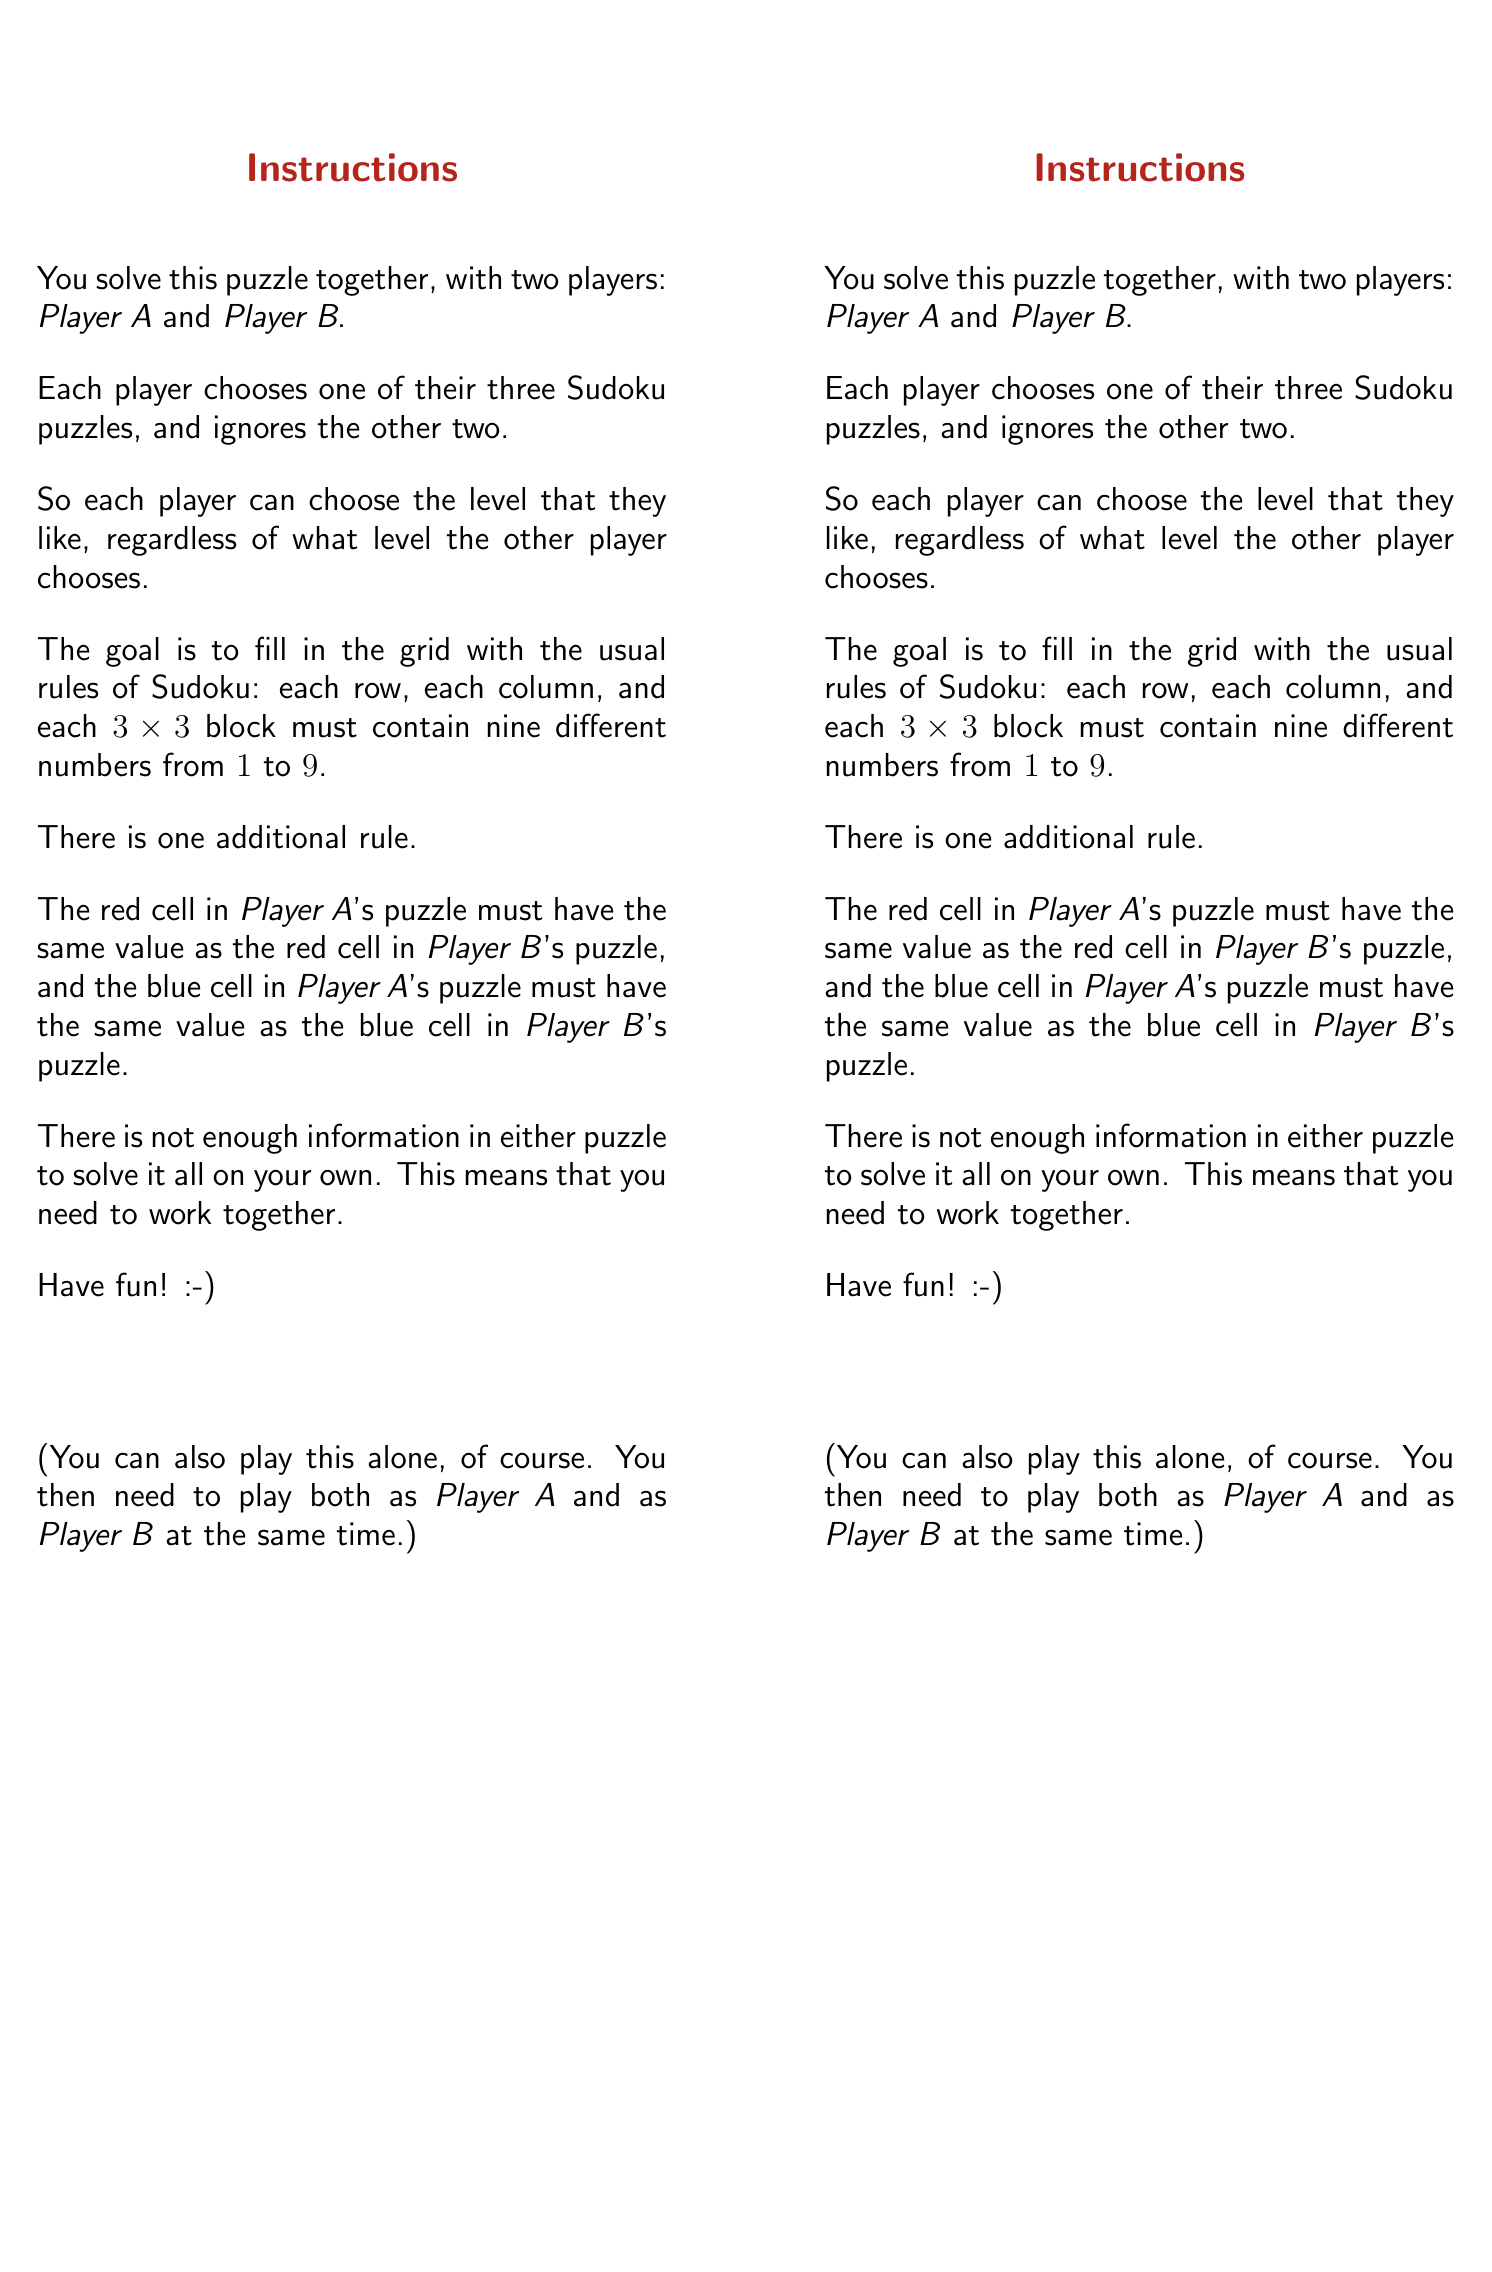
\begin{tikzpicture}
  %
  % PLAYER A
  \node[] at (-5,-1.25) {\parbox{5cm}{\centering \sffamily \Large \color{BrickRed} \textbf{Instructions}}};
  \node[] at (-5,-15) {\begin{minipage}[t][25.0cm][t]{8.0cm}\sffamily \large
  You solve this puzzle together, with two players: \textit{Player~A} and \textit{Player~B}.
  
  \bigskip
  
  Each player chooses one of their three Sudoku puzzles, and ignores the other two.
  
  \bigskip
  
  So each player can choose the level that they like,
  regardless of what level the other player chooses.
  
  \bigskip
  
  The goal is to fill in the grid with the usual rules of Sudoku:
  each row, each column, and each $3 \times 3$ block must contain
  nine different numbers from~$1$ to~$9$.
  
  \bigskip
  
  There is one additional rule.
  
  \bigskip
  
  The red cell in \textit{Player~A}'s puzzle must have the same value as the red
  cell in \textit{Player~B}'s puzzle,
  and the blue cell in \textit{Player~A}'s puzzle must have the same value as the blue
  cell in \textit{Player~B}'s puzzle.
  
  \bigskip
  
  There is not enough information in either puzzle to solve it all on your own.
  This means that you need to work together.
  
  \bigskip
  
  Have fun! :-)
  
  \bigskip\bigskip\bigskip\bigskip
  
  (You can also play this alone, of course. You then need to play both as
  \textit{Player~A} and as \textit{Player~B} at the same time.)
  
  \vfill
  \end{minipage}};
  % PLAYER B
  \node[] at (5,-1.25) {\parbox{5cm}{\centering \sffamily \Large \color{BrickRed} \textbf{Instructions}}};
  \node[] at (5,-15) {\begin{minipage}[t][25.0cm][t]{8.0cm}\sffamily \large
  You solve this puzzle together, with two players: \textit{Player~A} and \textit{Player~B}.
  
  \bigskip
  
  Each player chooses one of their three Sudoku puzzles, and ignores the other two.
  
  \bigskip
  
  So each player can choose the level that they like,
  regardless of what level the other player chooses.
  
  \bigskip
  
  The goal is to fill in the grid with the usual rules of Sudoku:
  each row, each column, and each $3 \times 3$ block must contain
  nine different numbers from~$1$ to~$9$.
  
  \bigskip
  
  There is one additional rule.
  
  \bigskip
  
  The red cell in \textit{Player~A}'s puzzle must have the same value as the red
  cell in \textit{Player~B}'s puzzle,
  and the blue cell in \textit{Player~A}'s puzzle must have the same value as the blue
  cell in \textit{Player~B}'s puzzle.
  
  \bigskip
  
  There is not enough information in either puzzle to solve it all on your own.
  This means that you need to work together.
  
  \bigskip
  
  Have fun! :-)
  
  \bigskip\bigskip\bigskip\bigskip
  
  (You can also play this alone, of course. You then need to play both as
  \textit{Player~A} and as \textit{Player~B} at the same time.)
  \vfill
  \end{minipage}};
  %
  \draw[] (0,0.5) edge[ultra thick, dashed,white] (0,-27);
  %
\end{tikzpicture}
\end{center}

\end{document}
